\section{ИССЛЕДОВАНИЕ РАБОТЫ РЕГИСТРА СДВИГА}

Микросхема имеет входы: тактовый (С), параллельной загрузки (D0 –
D3), выбора режима работы (S0 и S1), асинхронного сброса (R). Данные
также могут поступать в регистр в последовательном коде на входы DL
(при сдвиге влево) и DR (при сдвиге вправо). Все операции кроме сброса
выполняются в регистре синхронно по фронту тактовых импульсов. Внутренний код регистра может быть прочитан на выходах Q0 – Q3.

\begin{figure}[H]
	\centering
	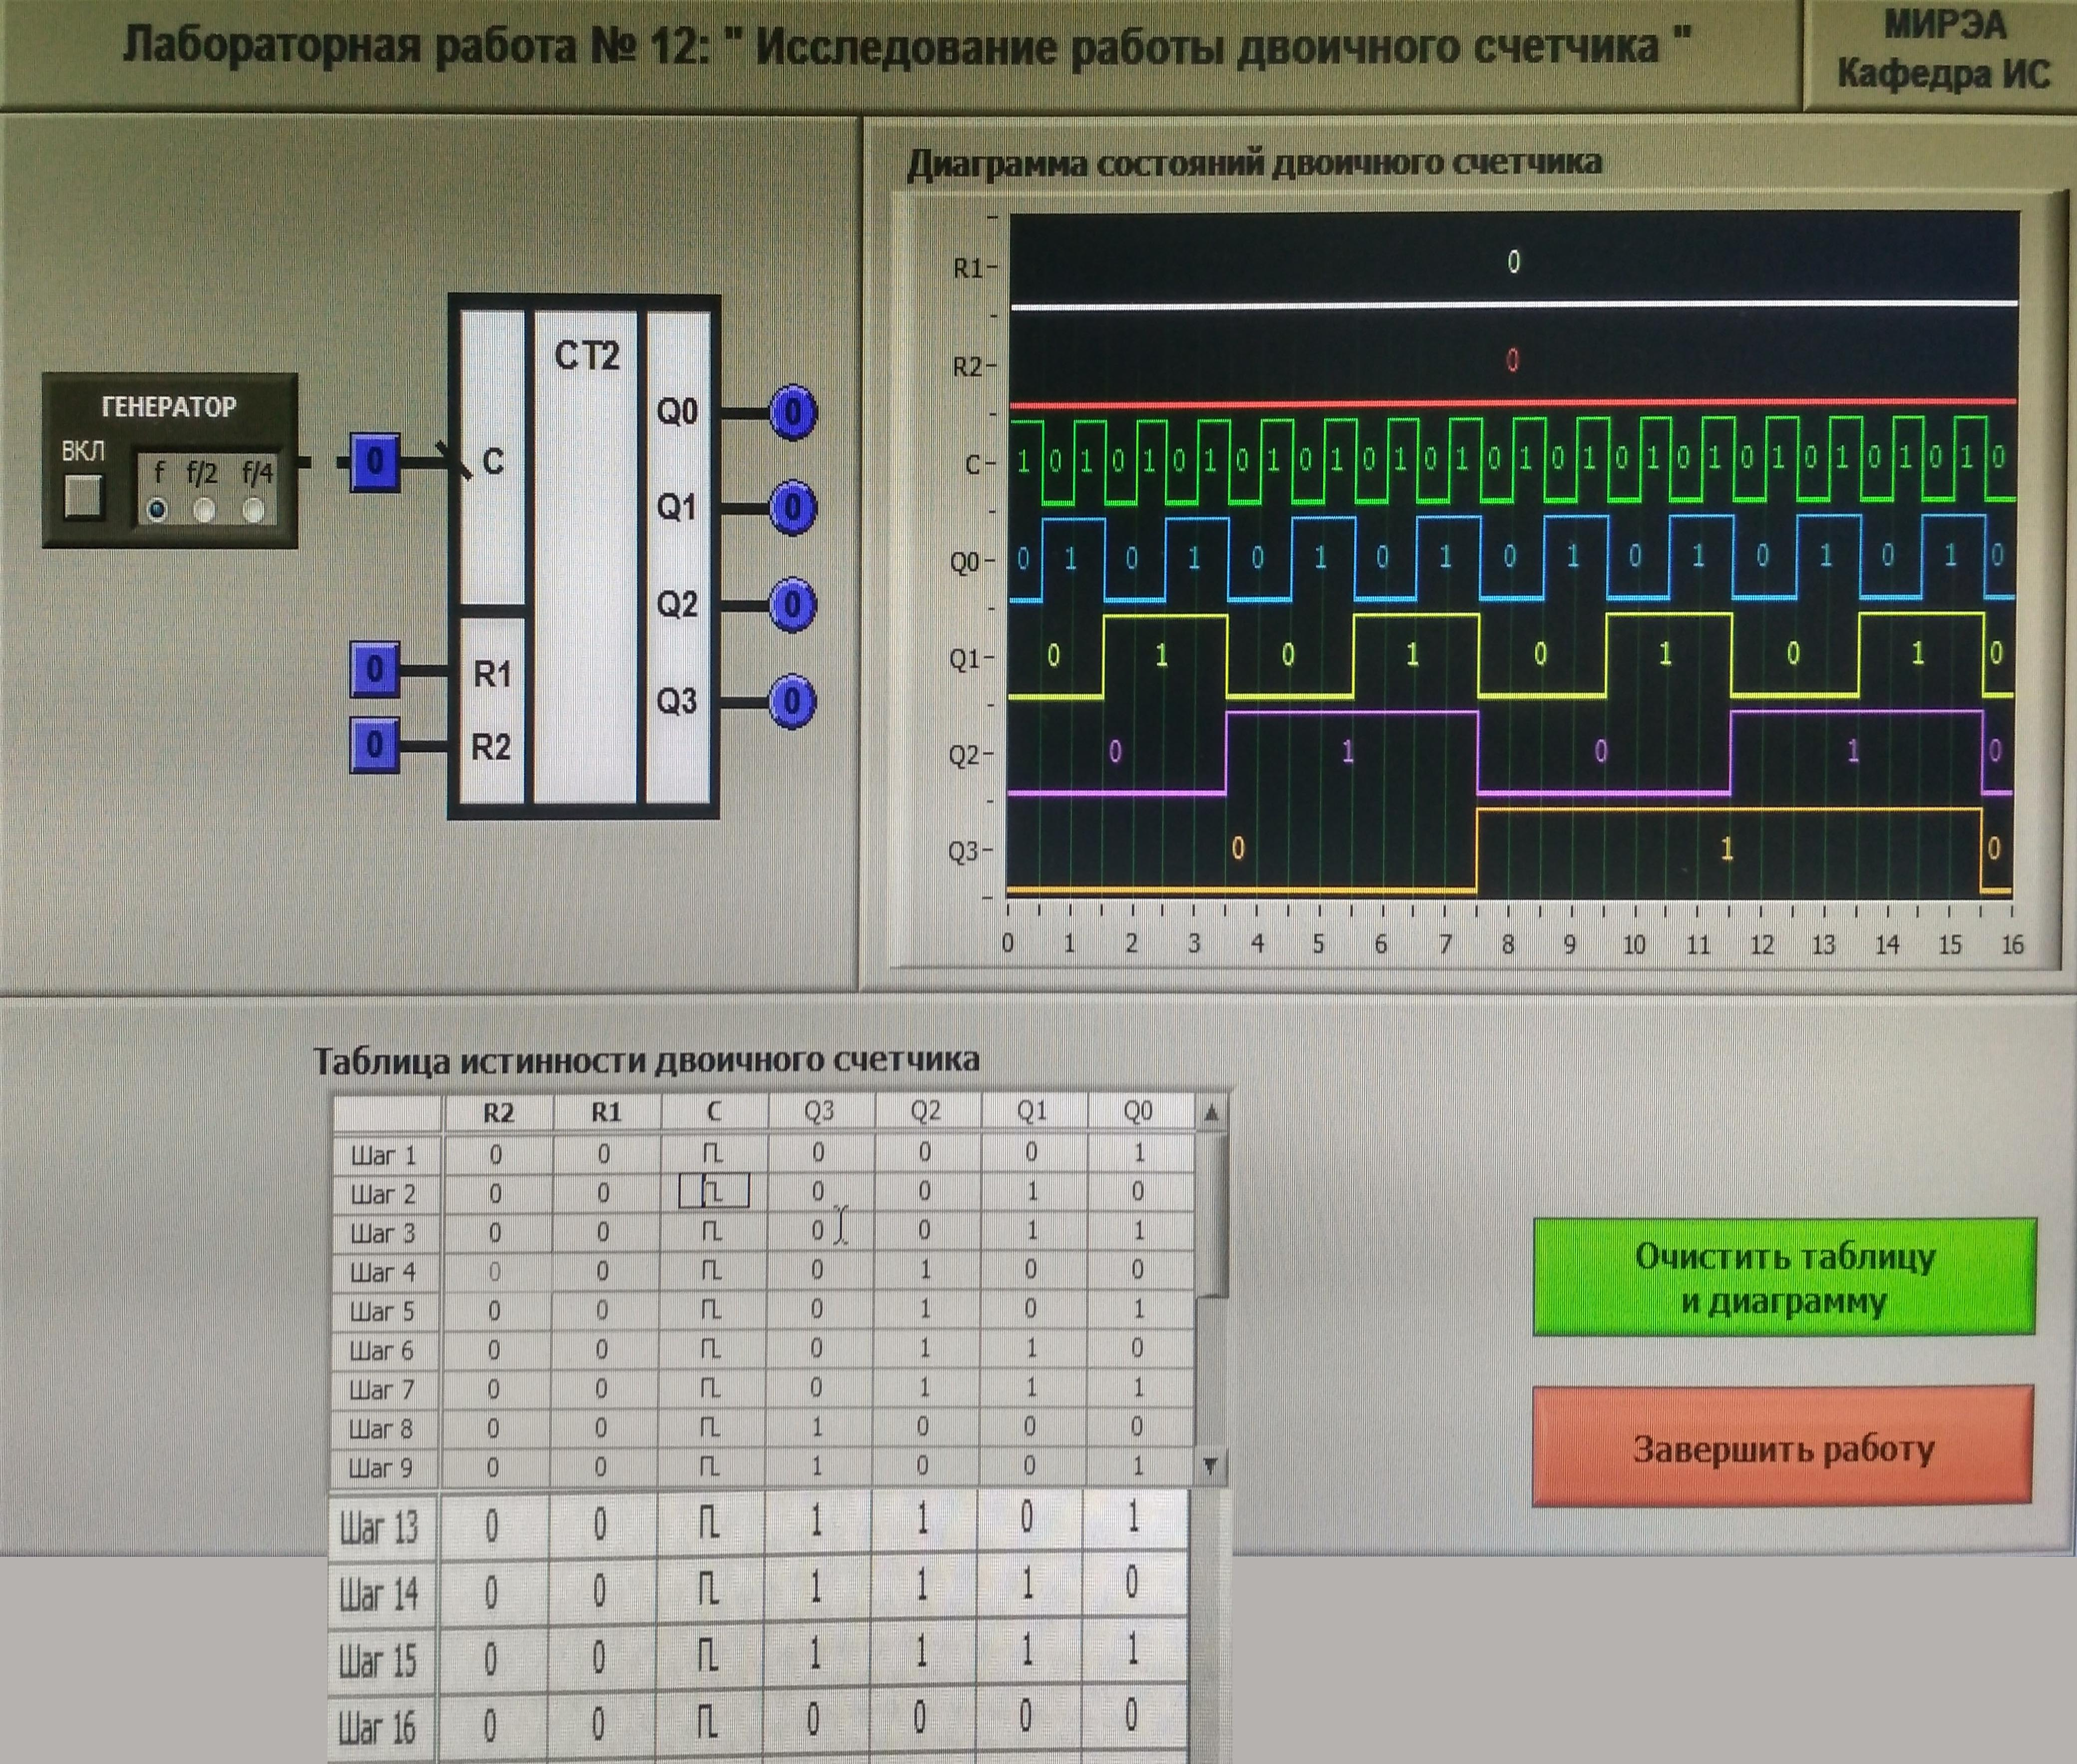
\includegraphics[width=0.95\linewidth]{imgs/11/1.jpg}
	\caption{РЕЖИМ СДВИГА ВПРАВО}
	\label{fig:11_1}
\end{figure}

\begin{figure}[H]
	\centering
	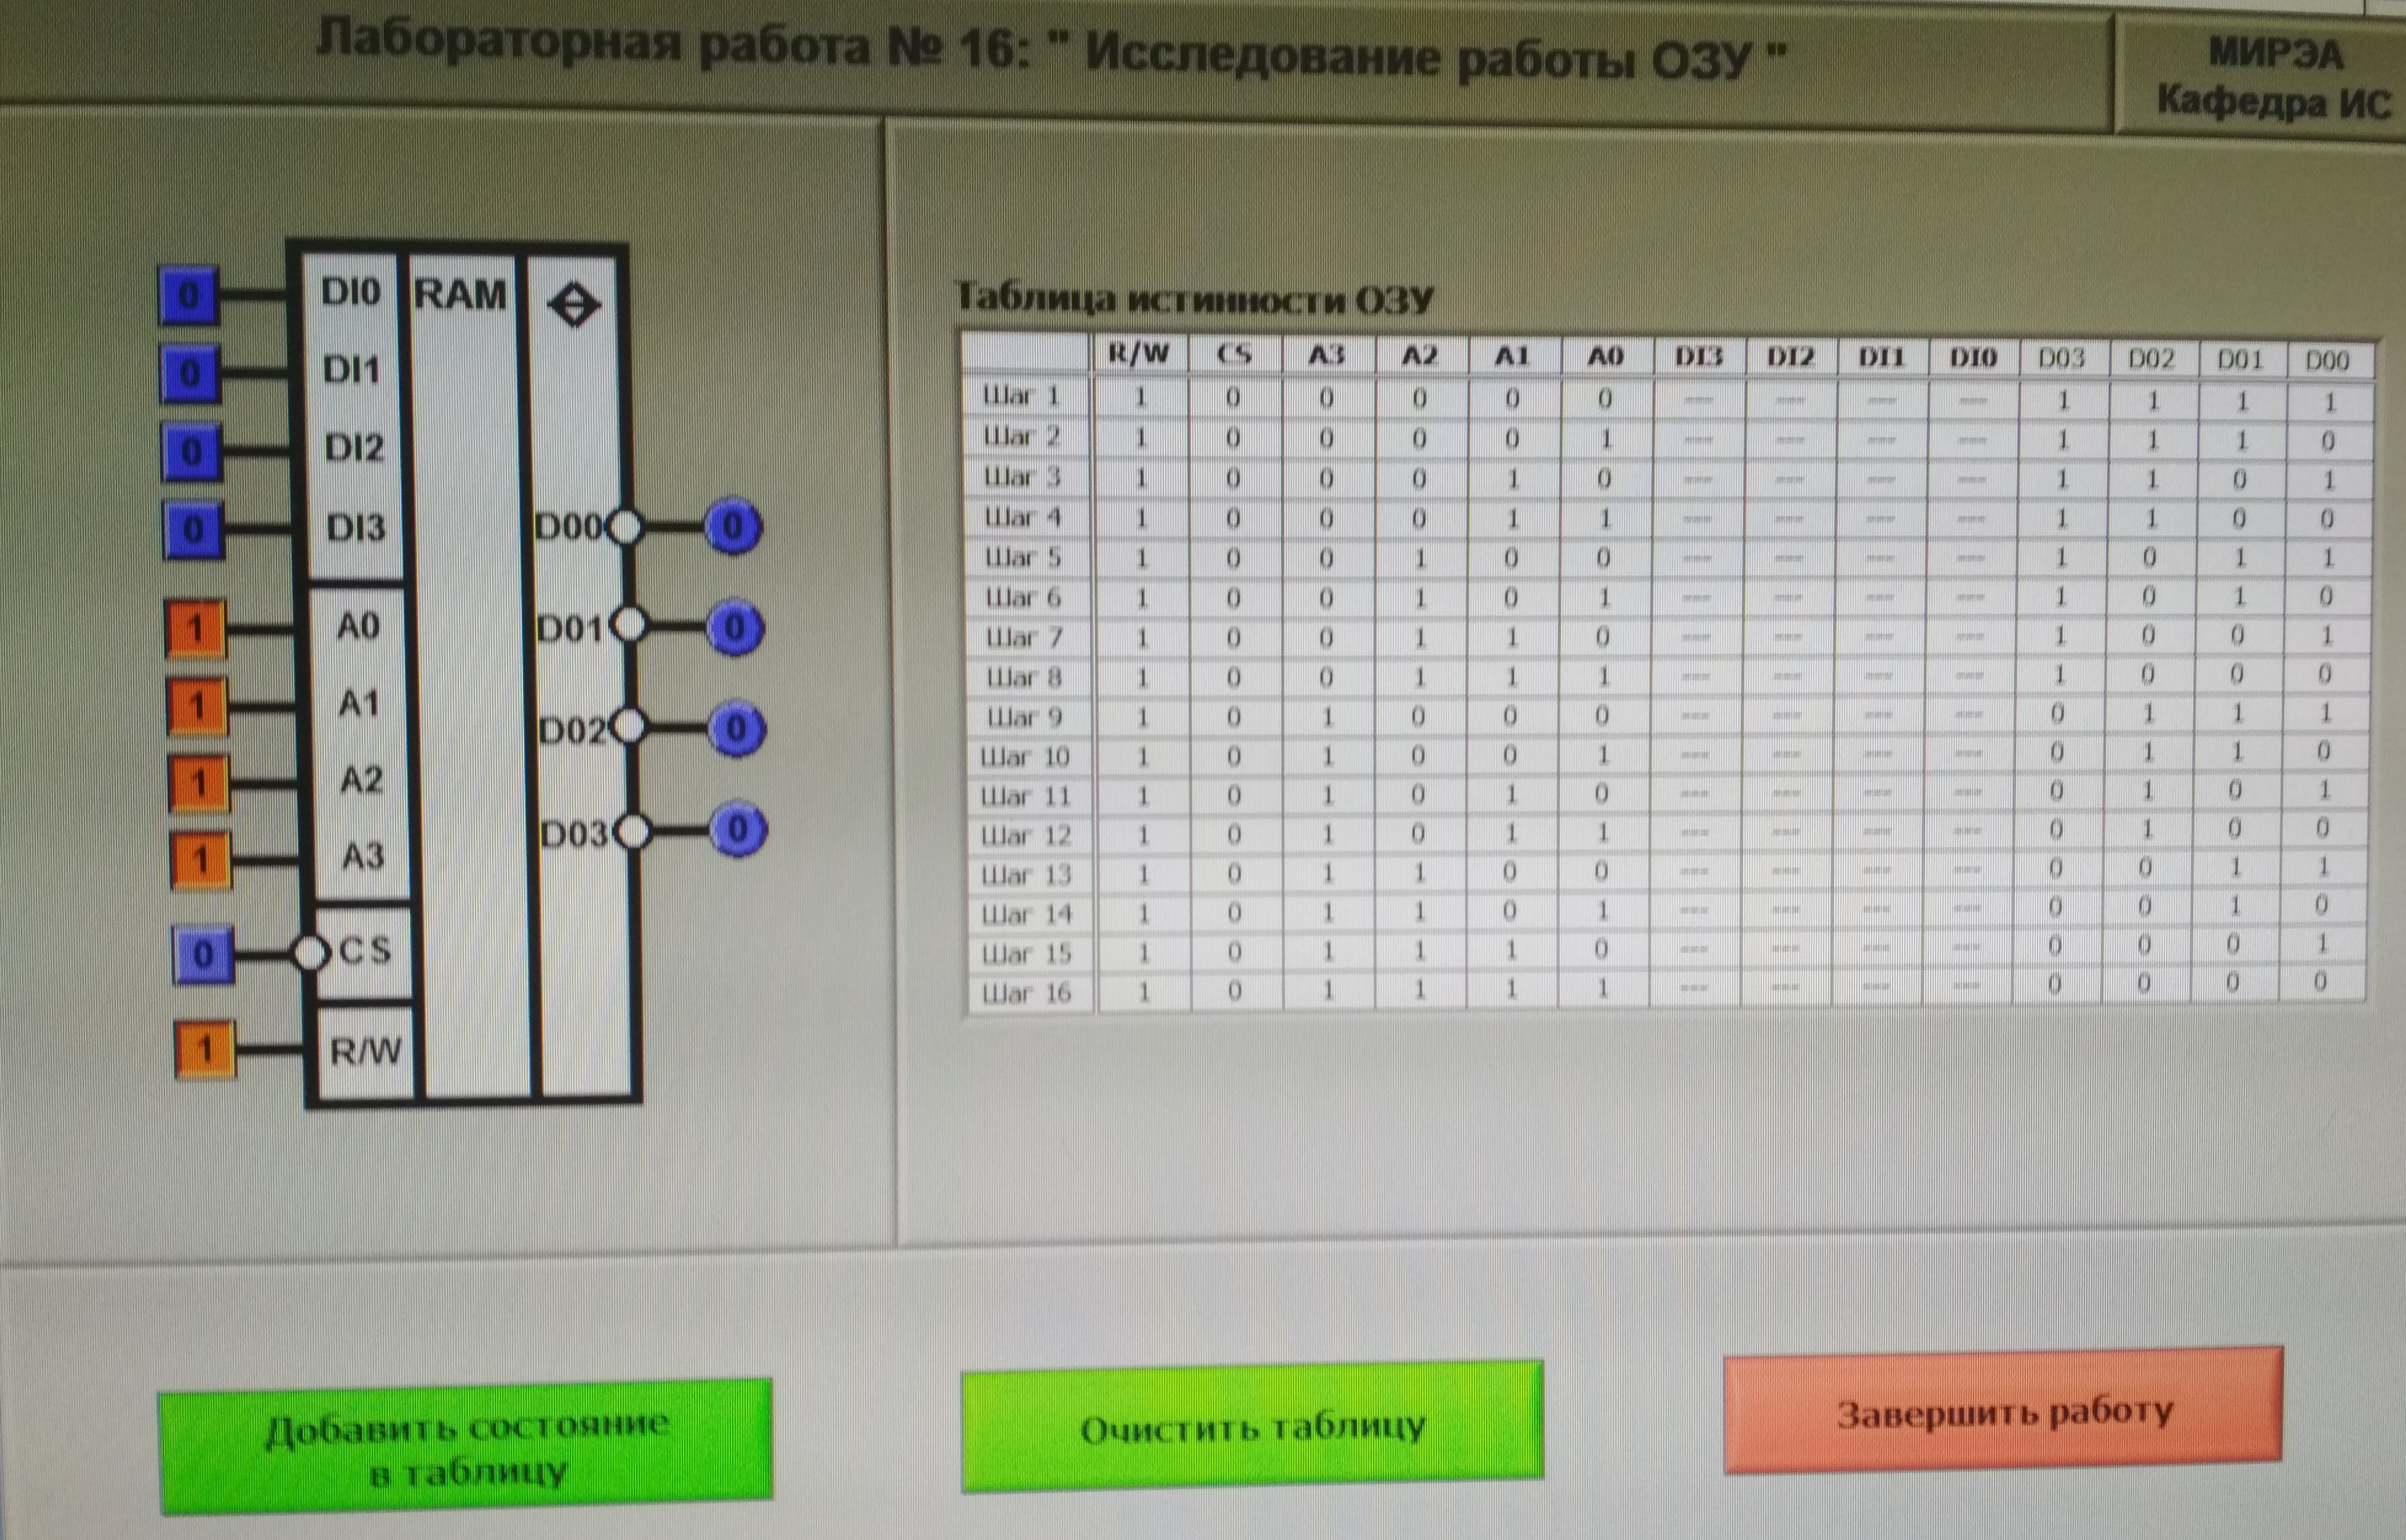
\includegraphics[width=0.95\linewidth]{imgs/11/2.jpg}
	\caption{РЕЖИМ СДВИГА ВЛЕВО}
	\label{fig:11_2}
\end{figure}

\begin{figure}[H]
	\centering
	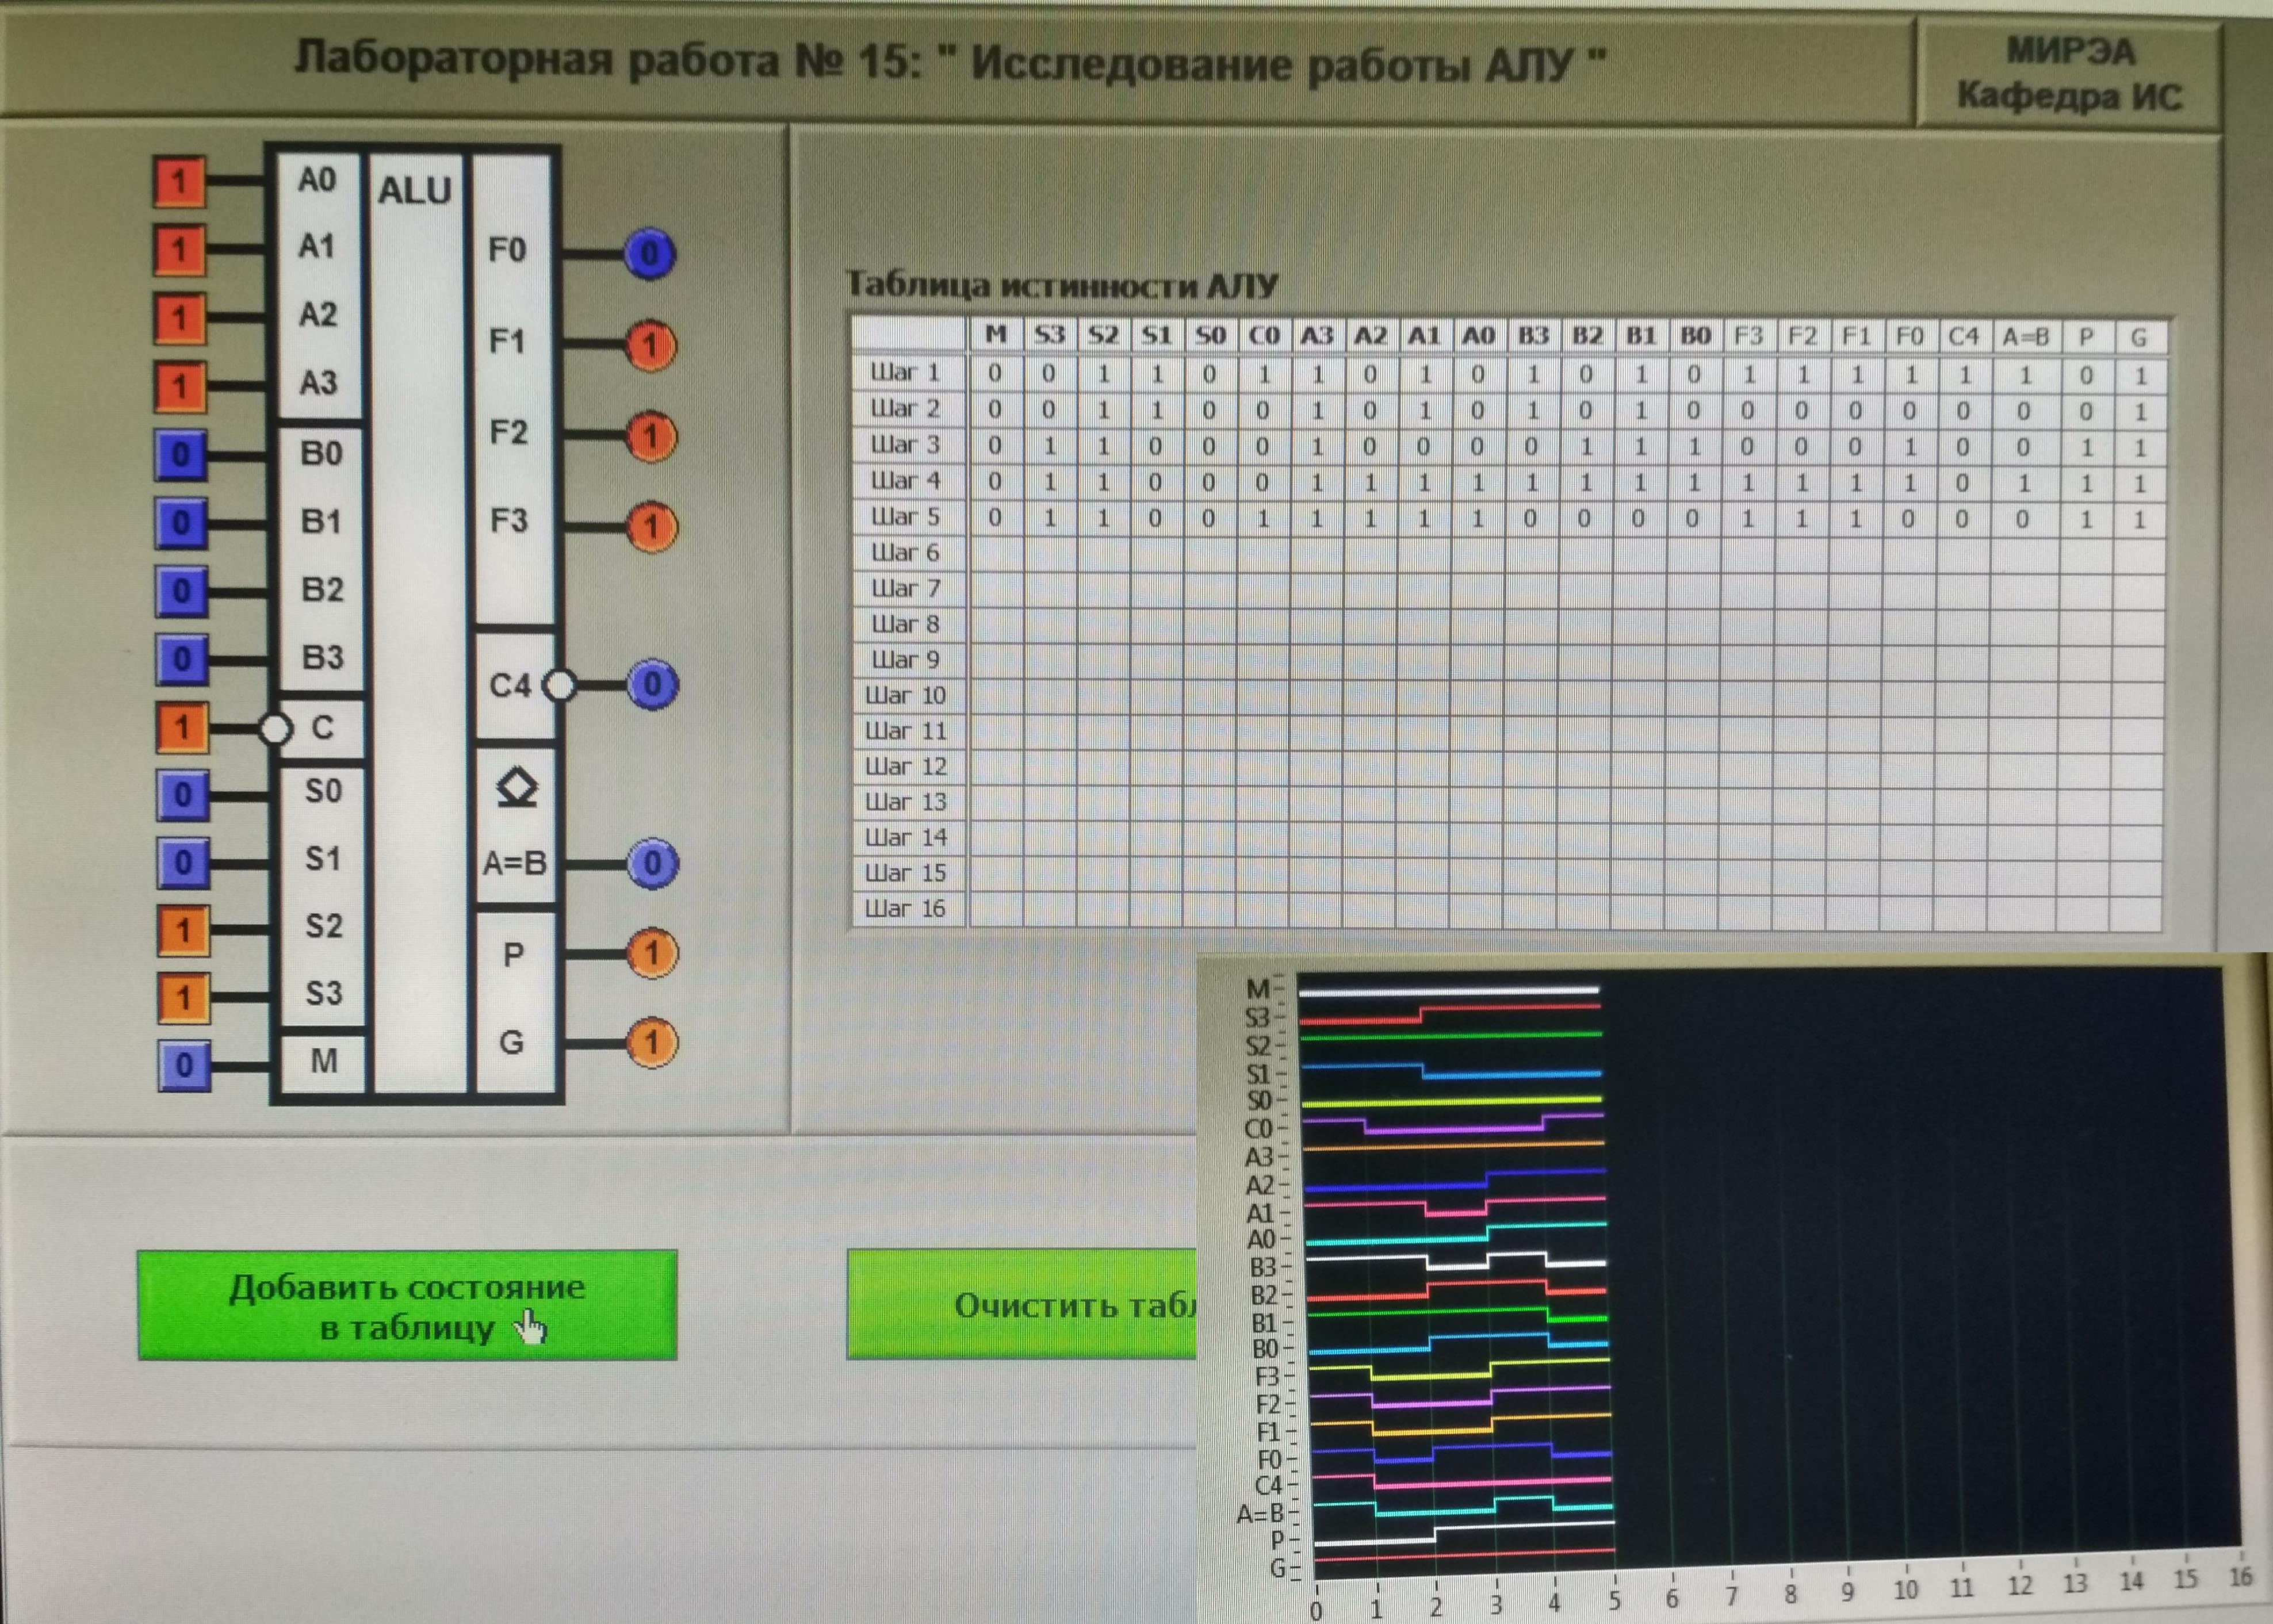
\includegraphics[width=0.95\linewidth]{imgs/11/3.jpg}
	\caption{РЕЖИМ ПАРАЛЛЕЛЬНОЙ ЗАГРУЗКИ}
	\label{fig:11_3}
\end{figure}

\begin{figure}[H]
	\centering
	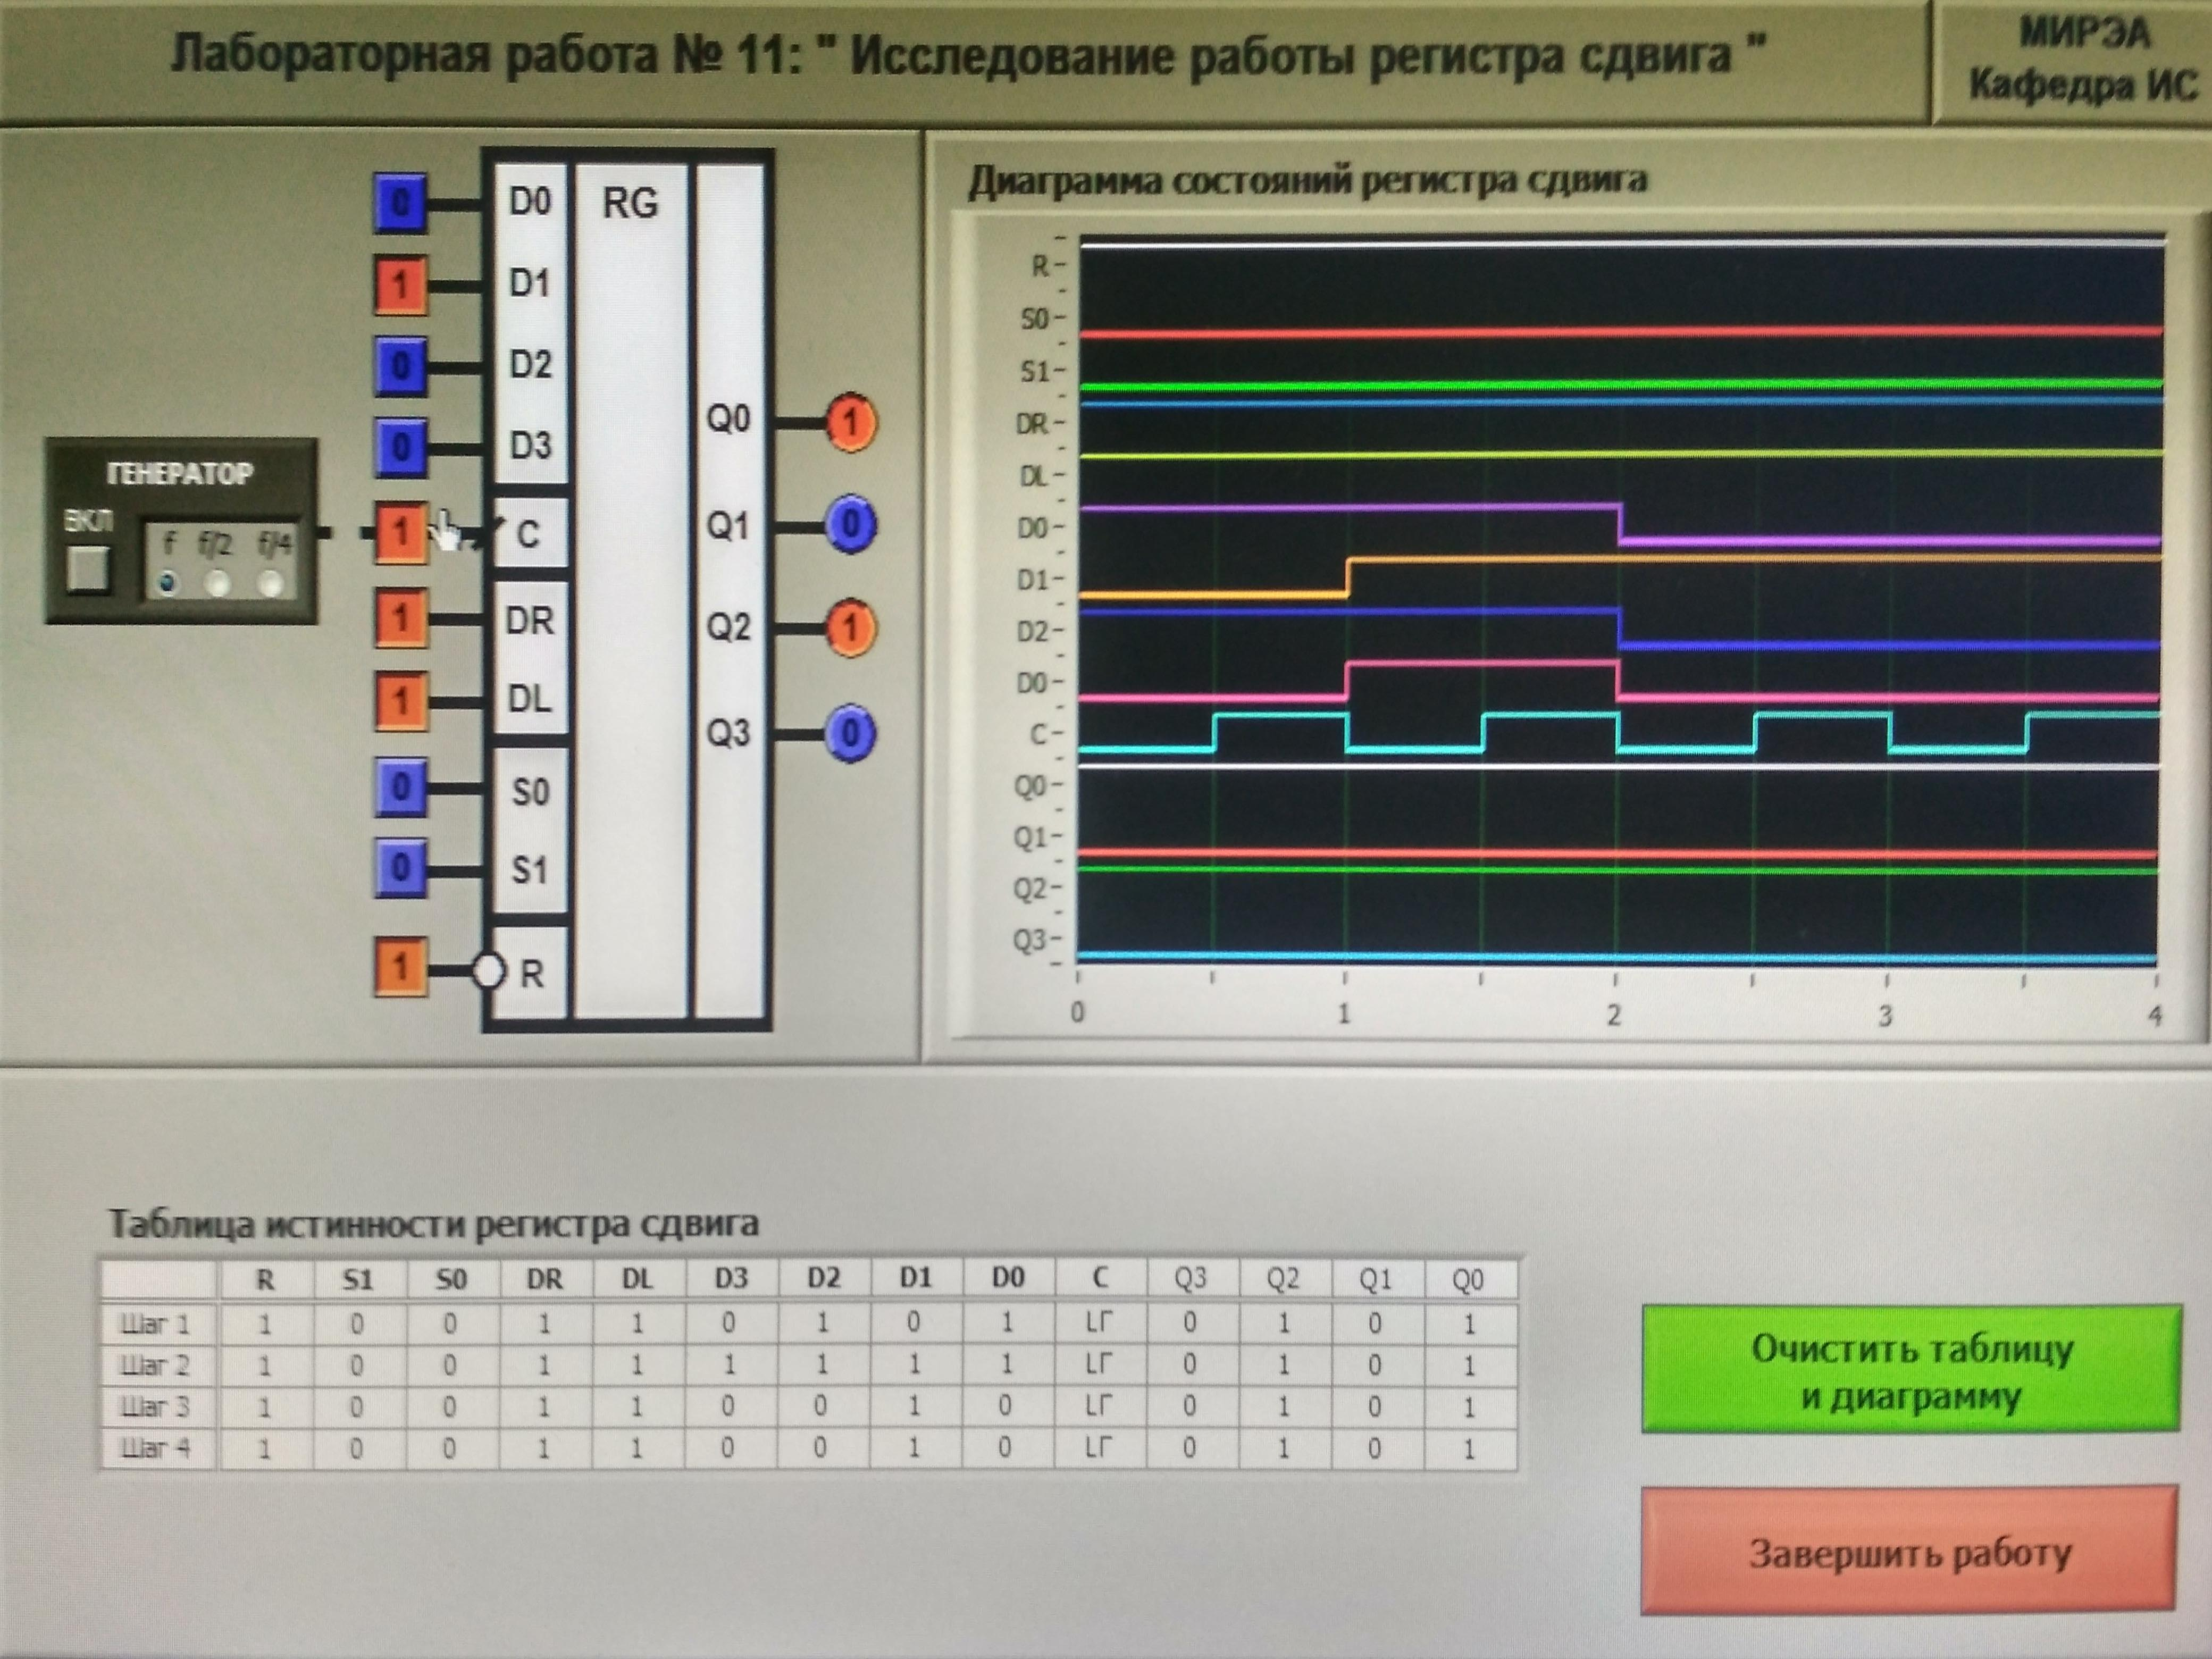
\includegraphics[width=0.95\linewidth]{imgs/11/4.jpg}
	\caption{РЕЖИМ ХРАНЕНИЯ}
	\label{fig:11_4}
\end{figure}


\begin{figure}[H]
	\centering
	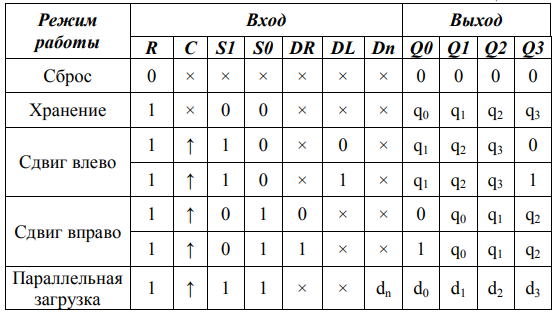
\includegraphics[width=0.85\linewidth]{imgs/11/11_tab}
	\caption{Режим работы регистра}
	\label{fig:11_tab}
\end{figure}

Элемент SN74LS194AN - Low-Voltage BiCMOS Technology

Характеристики:

Typical Shift Frequency of 36 MHz

\begin{figure}[H]
	\centering
	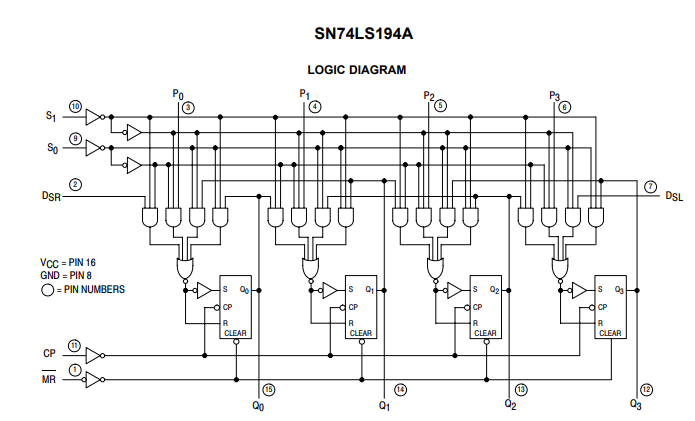
\includegraphics[width=0.95\linewidth]{imgs/11/11_sh}
	\caption{Схема}
	\label{fig:11_sh}
\end{figure}

\begin{figure}[H]
	\centering
	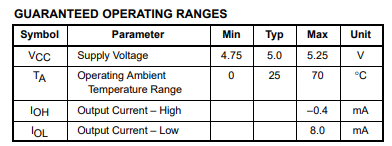
\includegraphics[width=0.95\linewidth]{imgs/11/11_guar}
	\caption{Рабочие параметры}
	\label{fig:11_guar}
\end{figure}

\begin{figure}[H]
	\centering
	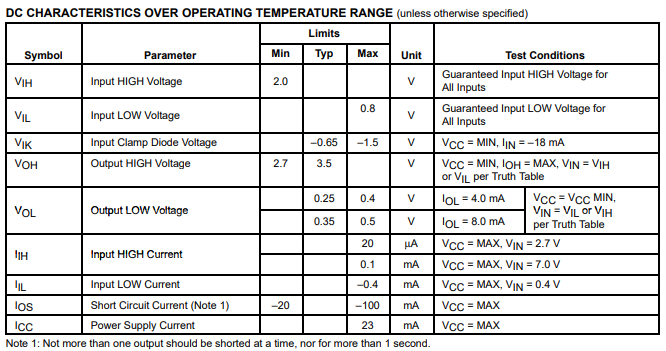
\includegraphics[width=0.95\linewidth]{imgs/11/11_dc}
	\caption{DC характеристики}
	\label{fig:11_dc}
\end{figure}

\begin{figure}[H]
	\centering
	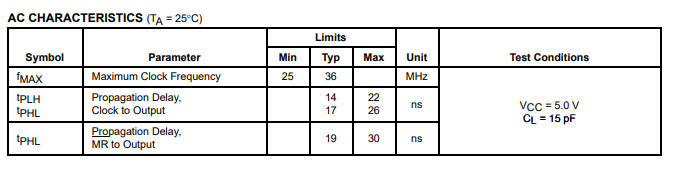
\includegraphics[width=0.95\linewidth]{imgs/11/11_ac_ch}
	\caption{AC характеристики}
	\label{fig:11_ac_ch}
\end{figure}
